\documentclass[10pt]{article}
\usepackage[margin=0.8in]{geometry}
\usepackage{amsmath,amssymb,graphicx,booktabs,array}
\usepackage[hidelinks]{hyperref}
\setlength{\parskip}{4pt}\setlength{\parindent}{0pt}
\newcommand{\E}{\mathbb E}

\title{Dose schedules on real data: a first evaluation}
\author{Claude, for Daniel Zou \quad (2026-10-28)}
\date{}

\begin{document}
\maketitle
\sloppy

\section*{What was done}

Twelve datasets were screened in which a dose is set by a known formula from an observed
score, $A=s(Q,\text{group})$. Each was run through the Model~2 estimator of
\texttt{dose\_schedule\_sketch.tex} (code: \texttt{experiments/methods/dose\_schedule.py};
runs: \texttt{experiments/scripts/dose\_schedule\_apply.py} and
\texttt{dose\_schedule\_figures.py}). The model is
\[
 \E\{Y(a)\mid X,\eta\}=\beta^\top X+g(\eta)+f(\eta,a)+(a-a_{\rm ref})\,\tau^\top Z,\qquad f(e,a_{\rm ref})=0,
\]
with a reference dose $a_{\rm ref}$ (zero, a floor or a cap) held by many units. The three role
rotations of the paper are used; nothing is tuned per dataset beyond the dose range.

\textbf{How to read each figure.}
\begin{itemize}
\item \textbf{Left, $\alpha$:} $\alpha_a(e)=\hat f(e,a)+(a-a_{\rm ref})\,\overline{\hat\tau^\top Z}$,
 the effect of dose $a$ against the reference dose for units with latent part $e$. Thick
 lines average the three rotations; thin lines are the rotations, so their spread shows the
 sampling noise. Solid where $e$ lies inside the 2.5--97.5\% range of $\hat\eta$ among units
 actually given a dose near $a$; dashed outside (extrapolation).
\item \textbf{Middle, $\psi$:} the transported average effect
 $\hat\psi(q,a)-\hat\psi(q,a_{\rm ref})$ for three score bins. Hollow markers: fewer than
 90\% of the bin's units lie inside the $\hat\eta$ range of that dose.
\item \textbf{Right, $U$:} $U(\theta)-U(\theta_0)$, the change in the mean outcome when every
 unit gets the dose of a one-parameter schedule $d_\theta$ instead of the status quo
 ($\theta_0$, dotted). The lower strip is the share of units whose new dose is supported for
 their $\hat\eta$. $U$ is the outcome change only: no dollar cost is subtracted, because each
 setting needs its own valuation (see the notes).
\end{itemize}

\section*{Summary}

\small
\begin{tabular}{>{\raggedright}p{2.6cm}>{\raggedright}p{3.6cm}rr>{\raggedright}p{5.2cm}}
\toprule
Dataset & Dose on score & $n$ & $R^2$ & Verdict\tabularnewline
\midrule
\textbf{UI, WA 1988 + IL 1984} & weekly benefit / cap on prior earnings; ref.\ the cap & 27,038 & 0.51 & \textbf{reasonable}: clean rule, stable average effect, two state schedules; small $n$\tabularnewline
\textbf{Medicare DSH, FY08--13} & DSH add-on (\%) on the low-income patient share; ref.\ 0 & 19,061 & 0.37 & \textbf{reasonable}: kinked schedule with a zero range, stable effects; thin outcomes\tabularnewline
\textbf{California LCFF, 2021--25} & concentration grant (\$/ADA) on the high-need share; ref.\ 0 & 10,645 & 0.82 & \textbf{reasonable}: kink at 55\%, high $R^2$; small $n$, persistent score\tabularnewline
NYC taxi, VTS + CMT & middle tip suggestion on the fare; ref.\ \$3 & 1,019,330 & 0.88 & mechanics excellent; flat $\alpha$, linear $U$, no cost\tabularnewline
Lending Club & interest rate on sub-grade; many rate tables & 171,175 & 0.40 & local only; selection on who borrows is missing\tabularnewline
E-Rate & discount (6 steps) on lunch share & 73,434 & 0.29 & local only; bunching at 49.5\%\tabularnewline
CMS dialysis QIP & payment cut (5 steps) on TPS & 57,328 & 0.46 & clean, but a null effect; large cuts rare\tabularnewline
Medicare Advantage & benchmark \% (steps) on FFS rank & 31,181 & 0.51 & clean, but noisy and near null\tabularnewline
NHANES school lunch & free/reduced/paid on income ratio & 12,730 & 0.31 & too small; eligibility, not take-up\tabularnewline
CMS readmissions & penalty from six ratios & 10,608 & 0.14 & several scores; not run\tabularnewline
Chile SEP; Title I & school / district funding steps & -- & -- & builds still running\tabularnewline
\bottomrule
\end{tabular}
\normalsize

\textbf{Two lessons.} (i) How far a dose can be moved along the score is limited by the
spread of $T=\hat\gamma^\top\tilde X$: with $R^2\approx0.3$--$0.4$ only neighbouring doses are
supported; with $R^2\approx0.8$--$0.9$ almost all are. (ii) The baseline $\beta^\top X$ carries
part of the identification, because units at high doses have covariates outside the range
of the reference units; with a cubic in distance the high-dose taxi estimates explode.

\newpage
\section*{1. Unemployment insurance (Upjohn bonus experiments)}

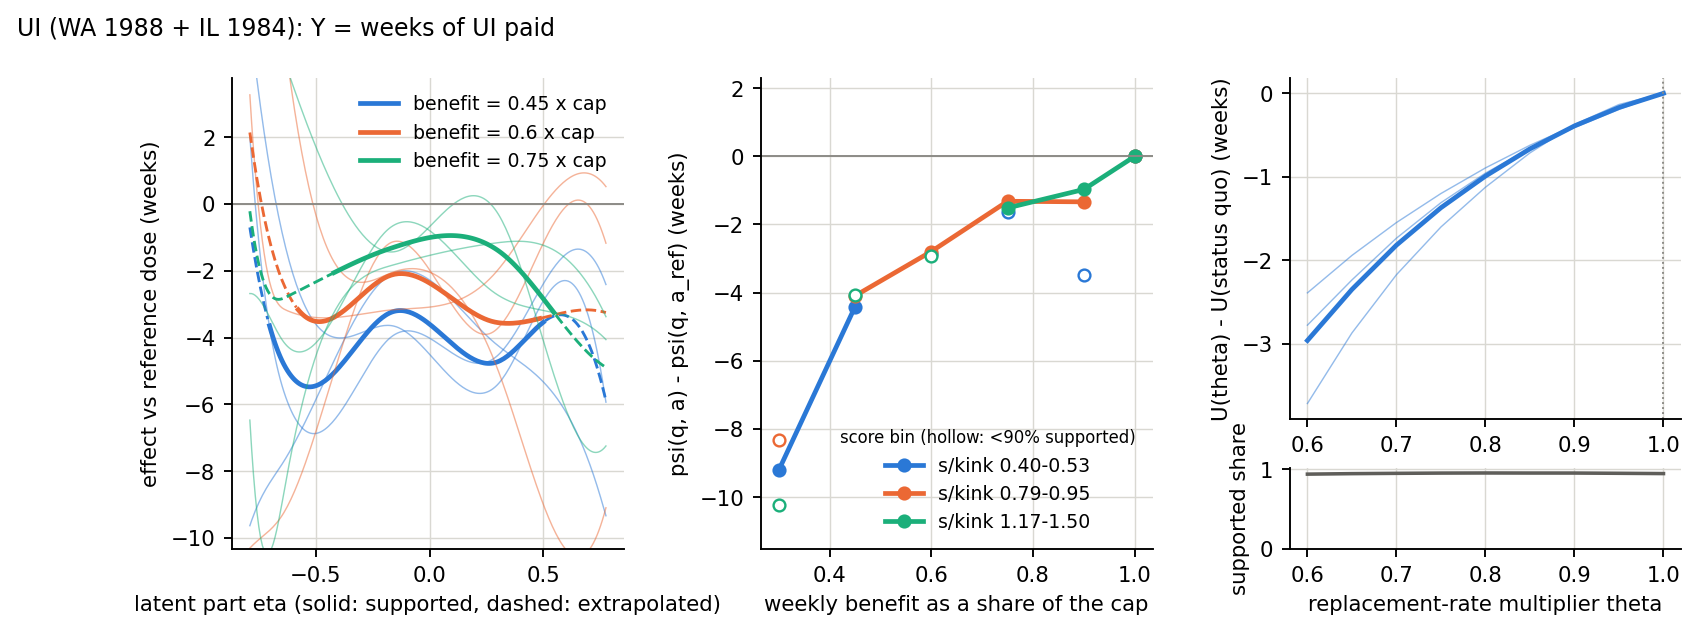
\includegraphics[width=\linewidth]{ui.png}

\begin{itemize}
\item \textbf{Setting.} Weekly benefit $=\text{rate}\times$ prior earnings between a floor and a
 cap (WA: 1/25 of the two-quarter average, cap \$205--209; IL: 48\%, cap \$161 plus
 dependents). The formula reproduces 94.7\% (WA) and 99.5\% (IL) of published benefits; no
 bunching at the kinks. Score: log(earnings / cap kink); 34\% of claimants are at the cap,
 which is the reference dose. Randomized bonus arms and state-period groups are in $X$.
\item \textbf{$\psi$:} at 60\% of the cap, weeks of UI paid fall by 2.7--3.2 against the cap in
 every supported earnings bin (mean 17.0 weeks), an elasticity of about 0.4, in line with
 the literature.
\item \textbf{$\alpha$:} negative at every $\eta$ but wiggly; the rotations disagree on its shape,
 so heterogeneity in $\eta$ is not determined with $n=27{,}038$.
\item \textbf{$U$:} scaling the replacement rate to $\theta=0.6$ (cap fixed) lowers weeks paid by
 3.0 (rotations 2.4--3.7) and benefits paid by \$1,001 per claimant (rotations \$923--1,065;
 mean \$2,339). A welfare $U$ needs a value of insurance (Baily--Chetty); with it, the interior
 optimum is the natural target.
\item \textbf{Next.} The five-state CWBH data (about 165,000 spells; your openICPSR login) would
 be the real application.
\end{itemize}

\section*{2. Medicare DSH adjustment}

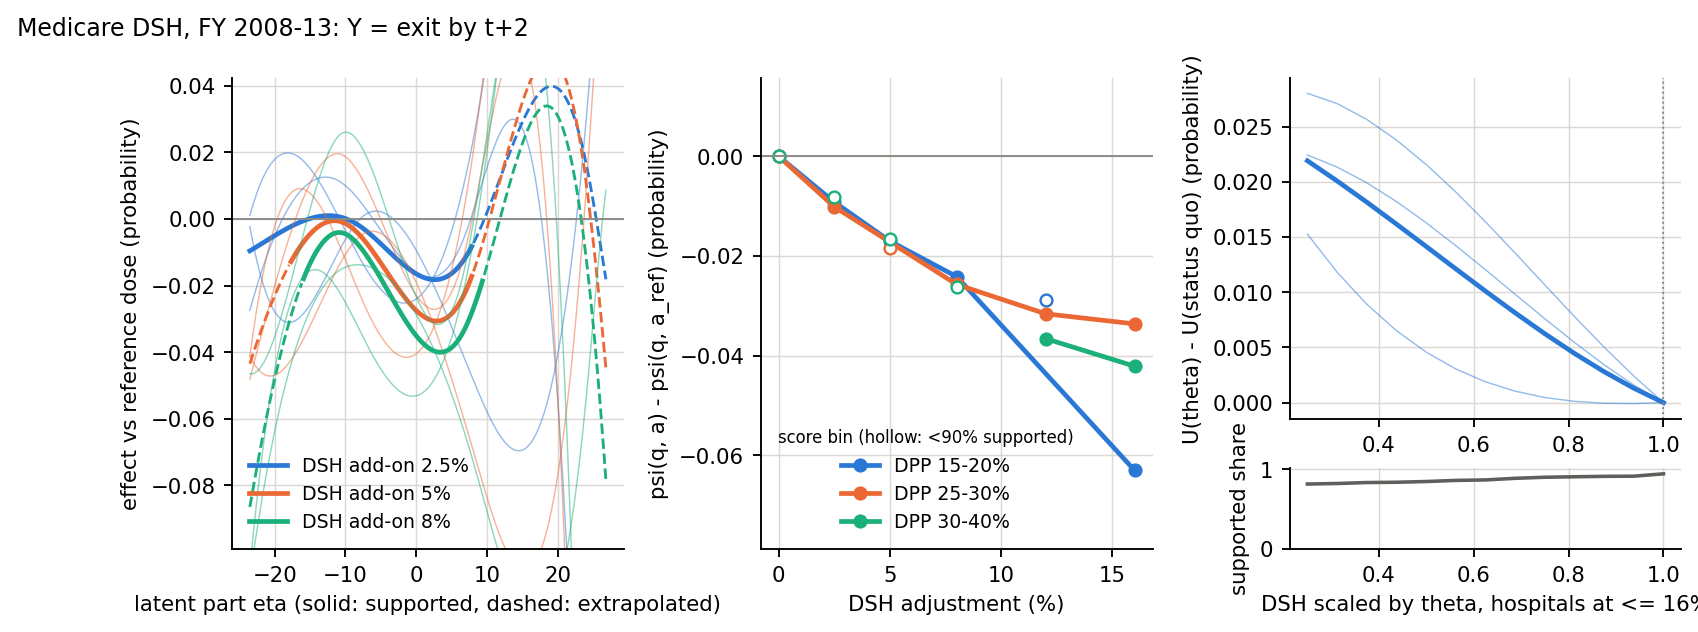
\includegraphics[width=\linewidth]{dsh_exit.png}
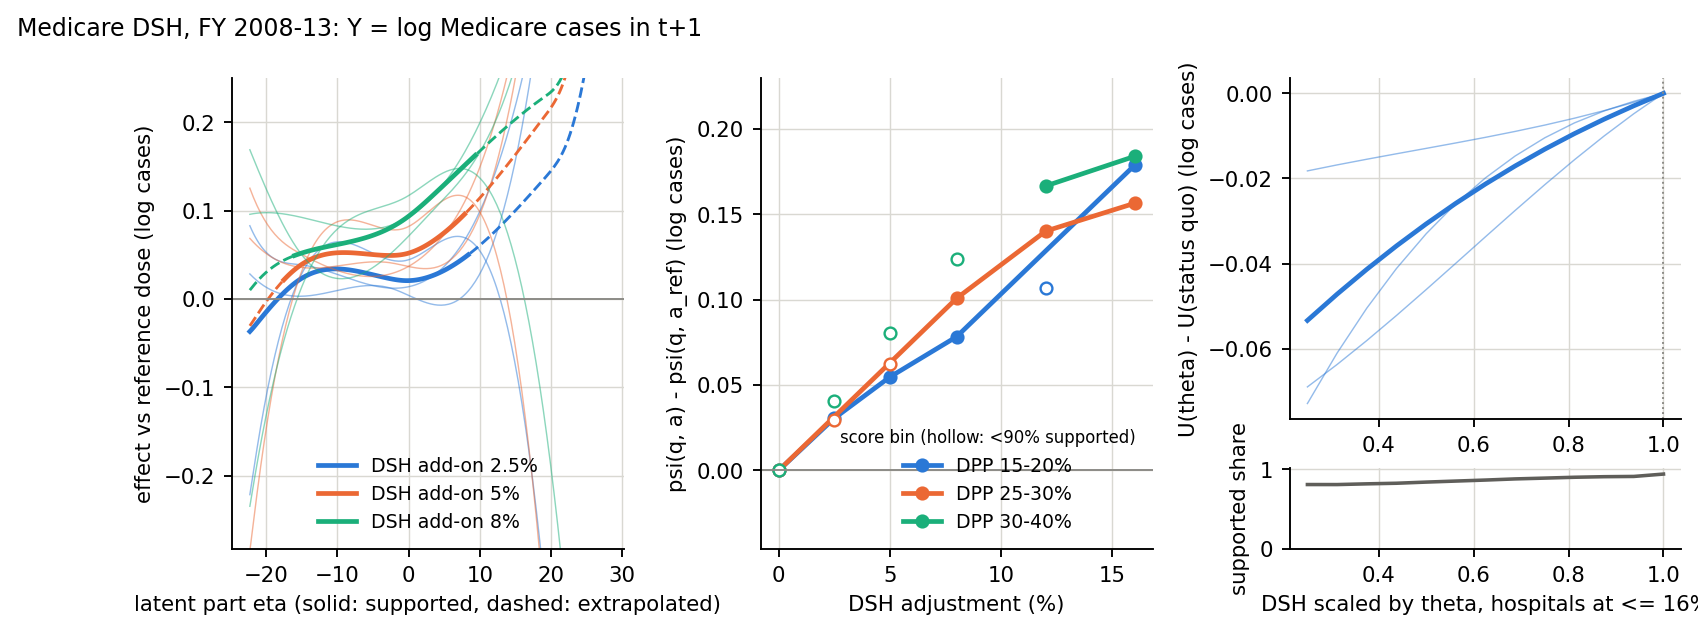
\includegraphics[width=\linewidth]{dsh.png}

\begin{itemize}
\item \textbf{Setting.} Add-on 0 below a 15\% low-income patient share, 2.5\% + 65\% of the excess
 up to 20.2\%, then 82.5\% of the excess; 12\% cap for small hospitals (a second schedule).
 Reproduced for every hospital-year 2007--2027 but one. FY 2014 cut the formula to 25\%.
\item \textbf{$\psi$:} closures fall and Medicare volume rises with the add-on, almost the same at
 each share bin: about $-1$ pp exit and $+3\%$ cases at 2.5\%, $-2.5$ pp and $+8$ to $+10\%$ at
 8\% (bins with a 15--30\% share, where these doses are supported).
\item \textbf{$U$:} cutting the formula to 25\% (the ACA's cut) for hospitals at $\le16\%$ raises
 exit by 2.2 pp (rotations 1.5--2.8; base rate 2.8\%) and lowers cases by 5.3\% (rotations
 1.8--7.3\%).
\item \textbf{Caveats.} The share is CMS's projection basis, not the settled one; mild excess mass
 just above 15\%; $\alpha$ in $\eta$ is noisy; financial outcomes need the HCRIS cost reports.
\end{itemize}

\section*{3. California LCFF concentration grant}

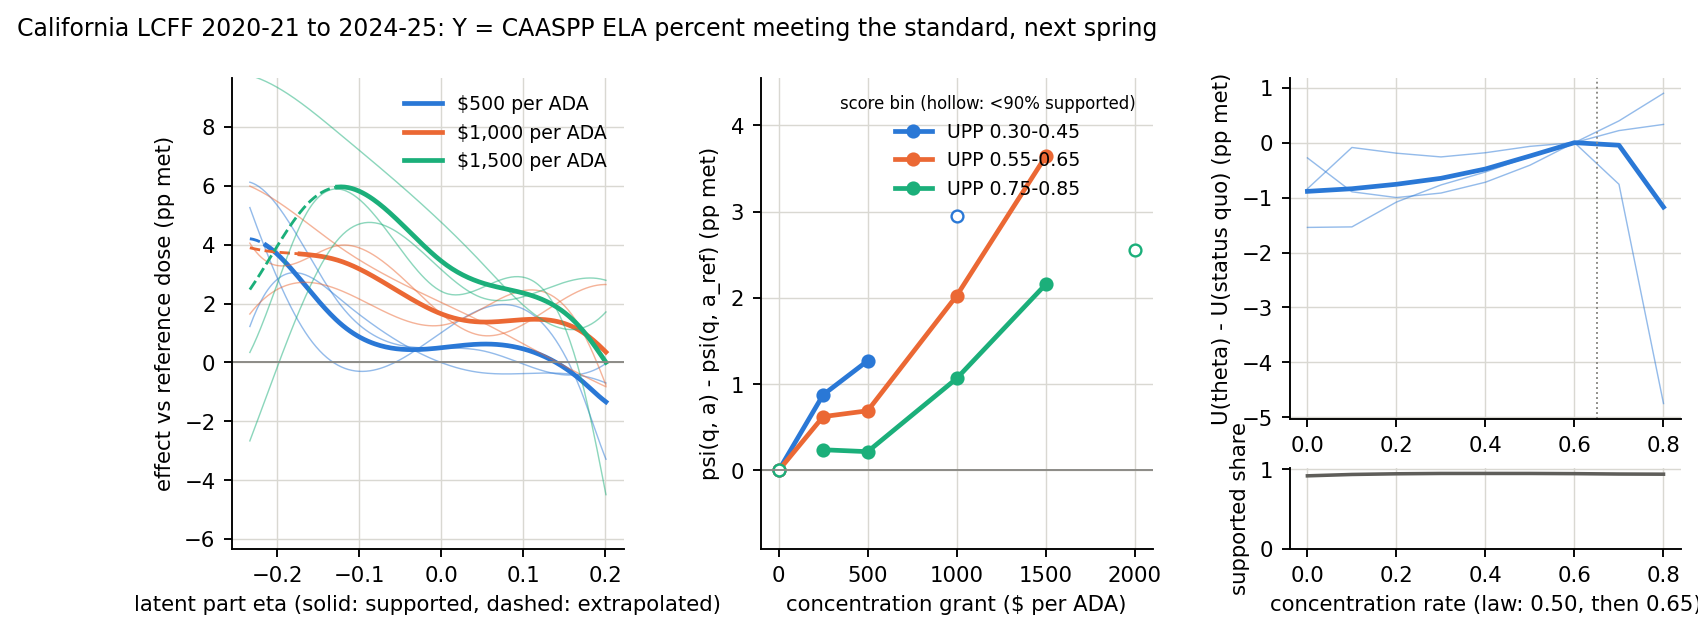
\includegraphics[width=\linewidth]{lcff.png}

\begin{itemize}
\item \textbf{Setting.} Grant per ADA $=c\times\text{base}\times\max(\text{UPP}-0.55,0)$ with
 $c=0.50$, then 0.65 from 2021--22; zero for 40\% of LEA-years. Reproduced to the dollar for
 all districts. No bunching at 55\%. Outcome: CAASPP percent meeting the standard the next
 spring; the lagged outcome is in $X$ and $Z$.
\item \textbf{$\psi$:} in the supported bins, \$1,000 per ADA raises ELA by 0.7--2.3 pp (math
 1.1--1.9), larger in the lower-need bins. Rotation spreads are 0.4--1.6 pp (ELA) and 1--2 pp (math).
\item \textbf{$U$:} see the right panel; removing the grant ($c=0$) lowers ELA by about 0.9 pp
 on average (rotations 0.3--1.5) and math by 1.1 pp (rotations $-0.1$ to 2.1); raising $c$ above 0.65 moves doses past the observed maximum.
\item \textbf{Caveats.} The score barely moves within an LEA; one year at $c=0.50$; COVID-era
 outcomes; charters' doses depend on another LEA's share.
\end{itemize}

\newpage
\section*{4. Mechanically strong, weak as policy problems}

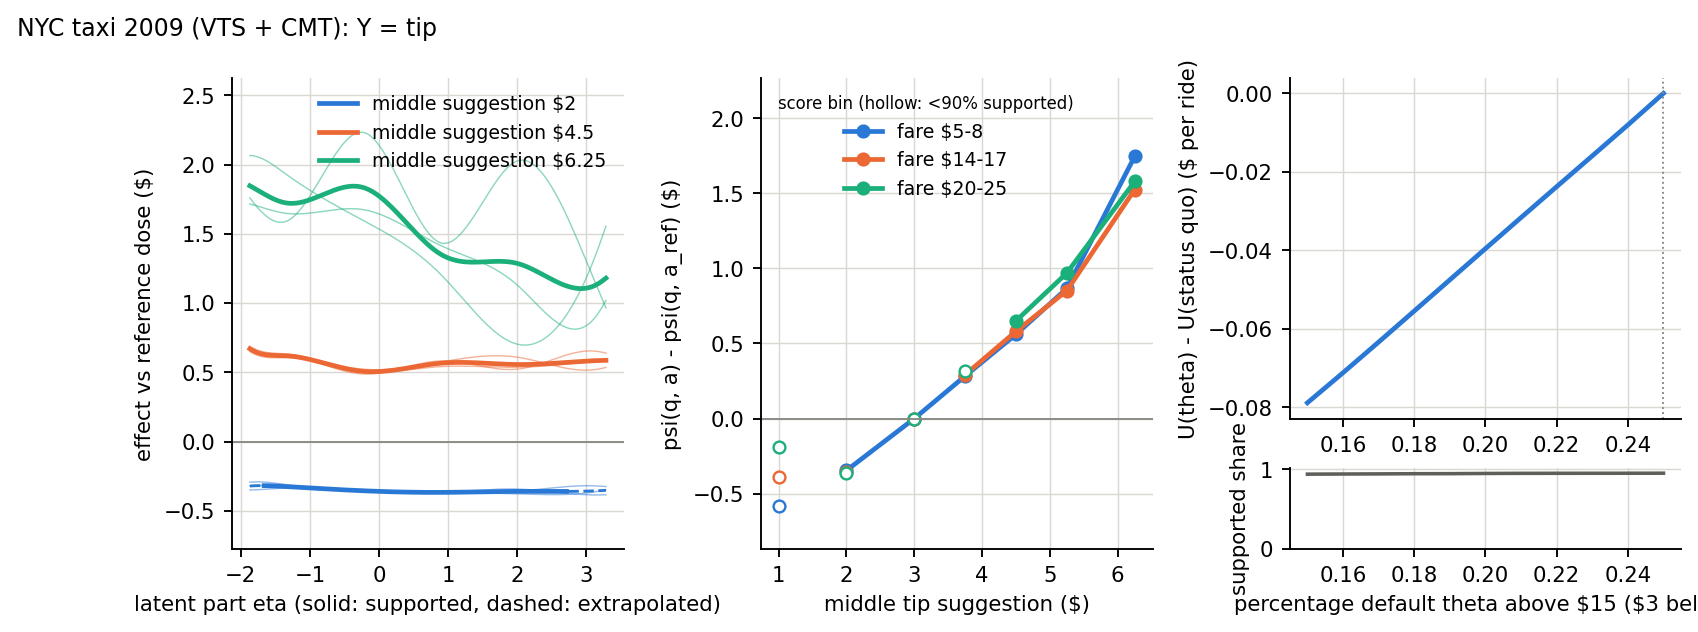
\includegraphics[width=\linewidth]{taxi2.png}

Taxi: two vendors give two schedules, $R^2=0.88$ and a million rides, so every dose is
supported. The tip rises by about \$0.35--0.40 per dollar of the middle suggestion, and
$\alpha$ is nearly flat in $\eta$. $U$ is linear in the default percentage and has no cost, so
there is no interior optimum. The score-direction modifier test rejects, possibly because the
two vendors' menus and fleets differ.

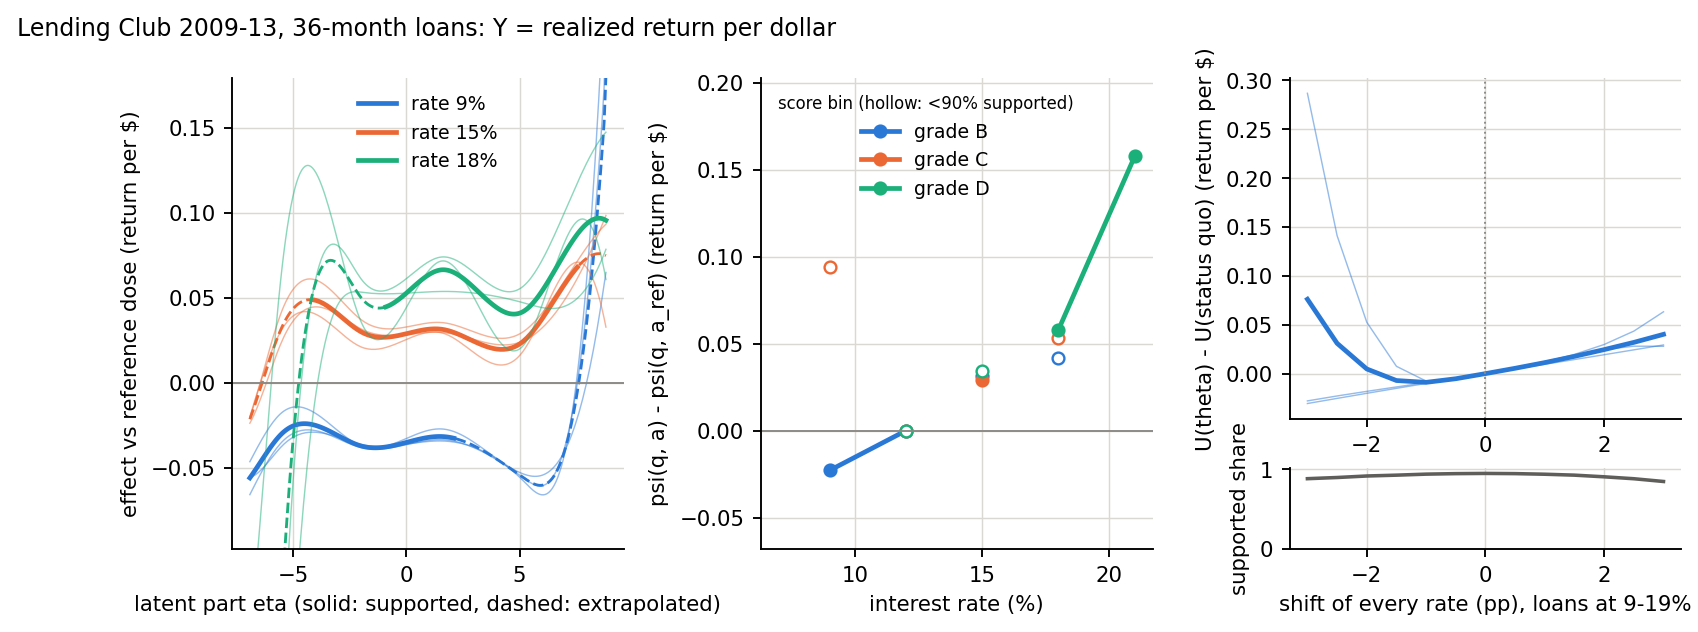
\includegraphics[width=\linewidth]{lending.png}

Lending Club: many rate tables over 2009--13 make the score-direction modifier testable (not
rejected). Realized return rises with the rate at every $\eta$, but only near each grade's own
rate is supported, and the data contain only loans that were taken, so the effect of a
higher rate on who borrows, the main force against raising rates, is missing.

\section*{Decisions for you}
\begin{itemize}
\item Which of UI, DSH and LCFF to develop. UI has the best policy story (optimal benefit
 schedule) but needs the CWBH download; DSH and LCFF are public and complete.
\item UI: reference dose at the cap (34\% of claimants, used here) or the floor (5\%).
\item LCFF: all LEAs (used here) or districts only; whether to add 2019--20.
\item CMS dialysis: another session has a duplicate \texttt{esrd\_qip/} folder.
\end{itemize}

\end{document}
